\chapter{SRS DOCUMENT} \label{ch:procedure}
\section*{Chapter 3}

\subsection*{User Story}

A User Story is a simple, concise description of a software feature told from the perspective of the end-user who desires the capability. It follows a standard template to capture the who, what, and why of a requirement:\\
\texttt{\"As a [type of user], I want to [perform some action] so that [I achieve some goal/benefit].\"}

    
\section{Functional Requirement 1: Vendor Registration, Subscription, and Secure Authentication}

\textbf{ID:} FR-01 \\
\textbf{Title:} Vendor Onboarding, Subscription Enforcement, and Two-Factor Authentication (2FA)\\
\textbf{Description}\\
The system shall provide a comprehensive registration workflow for new Vendors (Tenants). During sign-up, the system must enforce the collection of business verification documents and payment for a subscription plan. Post-registration, access to the system must be secured via Two-Factor Authentication.\\
\textbf{Specific Requirements}

\begin{table}[H]
\centering
\label{tab:vendor-requirements}
\begin{tabular}{>{\raggedright\arraybackslash}p{2cm}>{\raggedright\arraybackslash}p{3cm}>{\raggedright\arraybackslash}p{7cm}>{\centering\arraybackslash}p{2cm}}
\toprule
\textbf{ID} & \textbf{Requirement Title} & \textbf{Description} & \textbf{Priority} \\
\midrule
FR-01.1 & Data Collection & The system shall require the applicant to input the following mandatory fields: Full Name, Business Email, Phone Number, Physical Address, Shop Type (Category), and a strong Password. & High \\
\midrule
FR-01.2 & Document Verification & The system shall provide an interface for the applicant to upload digital copies of mandatory legal documents: E-TIN Certificate, Trade License/Certificate, and E-Return Submission Proof. & High \\
\midrule
FR-01.3 & Subscription Enforcement & Upon successful data entry and document upload, the system shall redirect the user to a payment gateway. The account creation process shall only be finalized after a successful subscription payment confirmation. & Critical \\
\midrule
FR-01.4 & 2FA Implementation & Upon every login attempt, the system shall enforce Two-Factor Authentication (2FA). The system will send a One-Time Password (OTP) to the vendor's registered email or phone number, which must be entered to access the dashboard. & High \\
\midrule
FR-01.5 & Account Activation & The account shall remain in a ``Pending'' state until the subscription is active. & Medium \\
\bottomrule
\end{tabular}
\end{table}

\section*{User Stories for FR-01: Vendor Onboarding}

\subsection*{User Story 1.1: Vendor Registration \& Document Upload}
\begin{itemize}
    \item \textbf{As a} new Entrepreneur (Prospective Vendor),
    \item \textbf{I want to} upload my Trade License, E-TIN, and business details during sign-up,
    \item \textbf{So that} my business is verified and I can legally operate my store on the platform.
\end{itemize}

\noindent\textbf{Acceptance Criteria:}
\begin{enumerate}
    \item The ``Sign Up'' button is disabled until all mandatory fields are filled.
    \item The system accepts PDF or Image files for Trade License, E-TIN, and E-Return.
    \item The system validates that the phone number and email are in the correct format.
\end{enumerate}

\vspace{1em}
\subsection*{User Story 1.2: Subscription Payment}
\begin{itemize}
    \item \textbf{As a} Prospective Vendor,
    \item \textbf{I want to} pay for a subscription plan using a digital payment gateway (e.g., bKash/Nagad) immediately after entering my details,
    \item \textbf{So that} my account can be activated and I can start setting up my shop.
\end{itemize}

\noindent\textbf{Acceptance Criteria:}
\begin{enumerate}
    \item User is redirected to the payment gateway after document upload.
    \item If payment fails, the user is returned to the payment screen with an error message.
    \item If payment succeeds, the user is redirected to the ``Registration Successful'' page.
\end{enumerate}

\vspace{1em}
\subsection*{User Story 1.3: Secure Login with 2FA}
\begin{itemize}
    \item \textbf{As a} Registered Vendor,
    \item \textbf{I want to} receive an OTP on my phone or email when I log in,
    \item \textbf{So that} no one else can access my shop's financial data and order history even if they guess my password.
\end{itemize}

\noindent\textbf{Acceptance Criteria:}
\begin{enumerate}
    \item After entering the correct username and password, a ``Verify OTP'' screen appears.
    \item An OTP is sent to the registered contact method within 10 seconds.
    \item Access is granted only if the entered OTP matches the generated code.
\end{enumerate}

% FUNTIONAL REQ: 02

\section{Functional Requirement 2: Multi-Tenant Data Isolation and Security}

\textbf{ID:} FR-02 \\
\textbf{Title:} Database-per-Tenant Architecture and Centralized Tenant Management\\
\textbf{Description}\\
The system shall utilize a Multi-Tenant architecture designed to ensure strict data isolation and security. The backend must distinguish between the "Central System Data" and "Individual Tenant Data" to prevent data leakage between competing businesses.\\
\textbf{Specific Requirements}
\begin{table}[H]
\centering
\label{tab:multi-tenant-requirements}
\begin{tabular}{>{\raggedright\arraybackslash}p{2cm}>{\raggedright\arraybackslash}p{3.5cm}>{\raggedright\arraybackslash}p{7cm}>{\centering\arraybackslash}p{2cm}}
\toprule
\textbf{ID} & \textbf{Requirement Title} & \textbf{Description} & \textbf{Priority} \\
\midrule
FR-02.1 & Central Database (Catalog DB) & The system shall maintain a master database that stores global system information, including Vendor Login Credentials, Subscription Status, Tenant Metadata (Name, Shop URL), and System Logs. & \textcolor{criticalcolor}{\textbf{Critical}} \\
\midrule
FR-02.2 & Isolated Tenant Databases & Upon the successful registration of a new vendor, the system shall automatically provision a distinct, isolated database (or isolated schema) dedicated solely to that vendor. & \textcolor{criticalcolor}{\textbf{Critical}} \\
\midrule
FR-02.3 & Data Segregation & The isolated tenant database must store all private business data, including Product Inventory, Customer Profiles, Order History, and Transaction Logs. & \textcolor{criticalcolor}{\textbf{Critical}} \\
\midrule
FR-02.4 & Routing Logic & The system middleware must identify the incoming request's origin (Tenant ID) and route the query dynamically to the correct isolated database. & \textcolor{criticalcolor}{\textbf{Critical}} \\
\midrule
FR-02.5 & Security Compliance & Cross-tenant SQL queries shall be strictly prohibited at the application level to ensure that Vendor A cannot access Vendor B's customer or sales data. & \textcolor{criticalcolor}{\textbf{Critical}} \\
\bottomrule
\end{tabular}
\end{table}


\section*{User Stories for FR-02: Multi-Tenant Architecture}

\subsection*{User Story 2.1: Automated Database Provisioning}
\begin{itemize}
    \item \textbf{As} the System (Super Admin),
    \item \textbf{I want to} automatically create a separate database for a new vendor immediately after their registration is approved,
    \item \textbf{So that} their data is physically or logically separated from other vendors from the very first moment.
\end{itemize}

\noindent\textbf{Acceptance Criteria:}
\begin{enumerate}
    \item When a ``New Tenant'' is created in the Master DB, a corresponding ``Tenant\_DB\_ID'' is created.
    \item The new database is initialized with the standard tables (Products, Orders, Customers) but contains zero data.
\end{enumerate}

\vspace{1em}
\subsection*{User Story 2.2: Data Privacy \& Isolation}
\begin{itemize}
    \item \textbf{As a} Vendor,
    \item \textbf{I want to} be assured that my customer list and best-selling products are stored in a database that other vendors cannot access,
    \item \textbf{So that} my business strategies and customer data remain confidential and secure.
\end{itemize}

\noindent\textbf{Acceptance Criteria:}
\begin{enumerate}
    \item A query made by Vendor A returning ``All Orders'' must strictly return only Vendor A's orders.
    \item System penetration tests confirm that data cannot leak from Tenant A to Tenant B.
\end{enumerate}

\vspace{1em}
\subsection*{User Story 2.3: Centralized Management}
\begin{itemize}
    \item \textbf{As the} Super Admin,
    \item \textbf{I want to} store all vendor login credentials and subscription expiry dates in a central master database,
    \item \textbf{So that} I can manage access control and billing for all users from a single dashboard without accessing their private shop data.
\end{itemize}

\noindent\textbf{Acceptance Criteria:}
\begin{enumerate}
    \item The Master Database contains a table of all registered Tenants.
    \item The Master Database does not contain specific product or order rows (these are in the tenant DBs).
\end{enumerate}


% FUN02 END
% FUNCTIONAL REQ: 3 Start
\section{Functional Requirement 03}

\textbf{ID:} OD-03 \\
\textbf{Title:} Offers and Discounts scheme creation.\\
\textbf{Description}\\
This feature will allow vendors to create offers and discounts for their customers that’ll help them develop marketing strategies and attract customers towards their business.
\\
\textbf{Specific Requirements}

\begin{table}[H]
\centering
\label{tab:vendor-requirements}
\begin{tabular}{>{\raggedright\arraybackslash}p{2cm}>{\raggedright\arraybackslash}p{3cm}>{\raggedright\arraybackslash}p{7cm}>{\centering\arraybackslash}p{2cm}}
\toprule
\textbf{ID} & \textbf{Priority} & \textbf{Requirement} \\
\midrule
OD-03.1 & High & The system shall allow Vendors to create percentage-based discounts (e.g., 10\% off) for individual products or entire categories. \\
\midrule
OD-03.2 & High & The system shall allow Vendors to set start and end dates/times for all discounts. \\
\midrule
OD-03.3 & Medium & The system shall allow Vendors to limit the number of times a discount can be used (e.g., first 50 customers).  \\
\midrule
OD-03.4 & Low & The system shall allow Vendors to create "Buy X Get Y" offers (e.g., Buy 2, Get 1 Free). \\
\bottomrule
\end{tabular}
\end{table}

\section*{User Stories for OD-03: }

\subsection*{US-03.1: Management of discounts and offers}
\begin{itemize}
    \item \textbf{As a} Vendor,
    \item \textbf{I want to} create a time-limited percentage discount for a product category,
    \item \textbf{So that} I can run a seasonal sale to boost sales.
\end{itemize}


\noindent\textbf{Acceptance Criteria:}
\begin{enumerate}
    \item Discount offers should be created properly.
    \item Offer scheduling should be done correctly.
    \item The customization process should be easy.
\end{enumerate}
% FUNCTIONAL REQ: 3 END
% FUNCTIONAL REQ: 4 Start
\section{Functional Requirement 04}

\textbf{ID:} TC-04 \\
\textbf{Title:} Themes and Interface Customization.\\
\textbf{Description}\\
This feature will allow vendors to customize the store’s interface using attractive themes and buttons. It will help the customer to operate through the page and make it user-friendly.

\\
\textbf{Specific Requirements}

\begin{table}[H]
\centering
\label{tab:vendor-requirements}
\begin{tabular}{>{\raggedright\arraybackslash}p{2cm}>{\raggedright\arraybackslash}p{3cm}>{\raggedright\arraybackslash}p{7cm}>{\centering\arraybackslash}p{2cm}}
\toprule
\textbf{ID} & \textbf{Priority} & \textbf{Requirement} \\
\midrule
TC-04.1 & High & The system shall provide Vendors with a dashboard to customize their storefront's primary color scheme.\\
\midrule
TC-04.2 & High & The system shall provide Vendors with a selection of pre-designed layout templates (e.g., grid, list) for product display.\\
\midrule
TC-04.3 & Medium & The system shall allow Vendors to create and manage a custom navigation menu for their storefront.  \\
\midrule
TC-04.4 & Low & The system shall allow Vendors to save multiple theme configurations as "presets" for quick switching. \\
\bottomrule
\end{tabular}
\end{table}

\section*{User Stories for TC-04: }

\subsection*{US-04.1: Store Theme Customization}
\begin{itemize}
    \item \textbf{As a} Vendor,
    \item \textbf{I want to} customize my store’s interface using some properties,
    \item \textbf{So that} my storefront has a unique and professional identity.
\end{itemize}

\noindent\textbf{Acceptance Criteria:}
\begin{enumerate}
    \item Enables sufficient customization.
    \item Makes the interface user-friendly.

\end{enumerate}

% FUNCTIONAL REQ: 4 End

%   FUNTIONAL REQUIREMENT 05 START

\section{Functional Requirement 5: Payment Gateway Integration and Order Payment Handling
}

\textbf{ID:} FR-05 \\
\textbf{Title:} Multi-Method Payment Processing and Cash on Delivery Support\\
\textbf{Description}\\
The system shall provide a secure and flexible payment mechanism that allows customers to complete purchases using multiple online payment gateways or Cash on Delivery (COD). The system must ensure proper payment verification before confirming orders while giving customers freedom to choose their preferred payment method.\\
\textbf{Specific Requirements}

\begin{table}[H]
\centering
\label{tab:payment-requirements}
\begin{tabular}{>{\raggedright\arraybackslash}p{2cm}>{\centering\arraybackslash}p{2cm}>{\raggedright\arraybackslash}p{10cm}}
\toprule
\textbf{ID} & \textbf{Priority} & \textbf{Description} \\
\midrule
FR-05.1 & High & The system shall support online payments via bKash, Nagad, Visa, and MasterCard, as well as Cash on Delivery (COD). \\
\midrule
FR-05.2 & Medium & The system shall allow customers to select their preferred payment method during checkout. \\
\midrule
FR-05.3 & High & For online payments, the system shall redirect the customer to the selected payment gateway and wait for payment confirmation before placing the order. \\
\midrule
FR-05.4 & Low & If COD is selected, the system shall place the order without online payment and mark the payment status as ``Pending (COD)''. \\
\midrule
FR-05.5 & High & The system shall update the order payment status as ``Paid'', ``Failed'', or ``Pending (COD)'' based on the transaction result. \\
\bottomrule
\end{tabular}
\end{table}

\section*{User Stories for FR-05: Payment Processing}

\subsection*{User Story 5.1: Choosing a Payment Method}
\begin{itemize}
    \item \textbf{As a} Customer,
    \item \textbf{I want to} choose between online payment and Cash on Delivery while placing an order,
    \item \textbf{So that} I can pay in the way that is most convenient for me.
\end{itemize}

\noindent\textbf{Acceptance Criteria:}
\begin{itemize}
    \item The checkout page displays all available payment options.
    \item The selected payment method is shown in the order summary.
    \item The order is successfully created based on the chosen payment method.
\end{itemize}

\vspace{1em}
\subsection*{User Story 5.2: Online Payment Confirmation}
\begin{itemize}
    \item \textbf{As a} Customer,
    \item \textbf{I want} my online payment to be verified before my order is confirmed,
    \item \textbf{So that} I am sure my payment has been successfully completed.
\end{itemize}

\noindent\textbf{Acceptance Criteria:}
\begin{itemize}
    \item The system redirects the user to the payment gateway.
    \item If payment fails, the order is not confirmed and an error message is shown.
    \item If payment succeeds, the order status is marked as ``Paid''.
\end{itemize}
%   END - FUNTIONAL REQUIREMENT 05 


%   START FUNTIONAL REQUIREMENT 06


\section{Functional Requirement 6: Product Delivery Tracking via Third-Party Logistics
}

\textbf{ID:} FR-06 \\
\textbf{Title:} Third-Party Courier Integration and Order Tracking
\\
\textbf{Description}\\
The system shall provide real-time product delivery tracking by integrating with third-party courier services such as Pathao or RedX using APIs. The platform itself shall not manage delivery operations but shall display shipment tracking information to customers and vendors within the system.\\
\textbf{Specific Requirements}

\begin{table}[H]
\centering
\label{tab:delivery-requirements}
\begin{tabular}{>{\raggedright\arraybackslash}p{2cm}>{\centering\arraybackslash}p{2cm}>{\raggedright\arraybackslash}p{10cm}}
\toprule
\textbf{ID} & \textbf{Priority} & \textbf{Description} \\
\midrule
FR-06.1 & \textcolor{highcolor}{\textbf{High}} & The system shall integrate with third-party delivery services (e.g., Pathao, RedX) using APIs. \\
\midrule
FR-06.2 & \textcolor{highcolor}{\textbf{High}} & Upon order confirmation, the system shall generate shipment requests through the selected courier service API. \\
\midrule
FR-06.3 & \textcolor{mediumcolor}{\textbf{Medium}} & The system shall retrieve delivery status updates such as Picked Up, In Transit, and Delivered from the courier API. \\
\midrule
FR-06.4 & \textcolor{highcolor}{\textbf{High}} & Customers shall be able to view delivery status directly from their order details page without visiting external courier websites. \\
\midrule
FR-06.5 & \textcolor{highcolor}{\textbf{High}} & Vendors shall be able to view delivery progress for each order from their dashboard. \\
\bottomrule
\end{tabular}
\end{table}

\section*{User Stories for FR-06: Delivery Service Integration}

\subsection*{User Story 6.1: Customer Delivery Tracking}
\begin{itemize}
    \item \textbf{As a} Customer,
    \item \textbf{I want to} track my order delivery from the platform itself,
    \item \textbf{So that} I do not need to visit the courier service's website separately.
\end{itemize}

\noindent\textbf{Acceptance Criteria:}
\begin{itemize}
    \item The order details page displays the current delivery status.
    \item Tracking data is fetched from Pathao or RedX APIs.
    \item Delivery status updates automatically as the shipment progresses.
\end{itemize}

\vspace{1.5em}
\subsection*{User Story 6.2: Vendor Delivery Monitoring}
\begin{itemize}
    \item \textbf{As a} Vendor,
    \item \textbf{I want to} see the delivery status of customer orders,
    \item \textbf{So that} I can respond to customer queries and manage order fulfillment efficiently.
\end{itemize}

\noindent\textbf{Acceptance Criteria:}
\begin{itemize}
    \item Vendors can view shipment status for each order.
    \item The system displays courier-provided tracking information accurately.
\end{itemize}


%   END - FUNTIONAL REQUIREMENT 06





% FUNCTIONAL REQUIREMENT 07 START
\section{Functional Requirement 07}

\textbf{ID:} IM-07\\
\textbf{Title:} Inventory Management\\
\textbf{Description}\\
This feature provides vendors with full control over their product life-cycle and stock accuracy, ensuring the digital storefront remains synchronized with physical availability.\\
\textbf{Specific Requirements}

\begin{table}[H]
\centering
\label{tab:vendor-requirements}
\begin{tabular}{>{\raggedright\arraybackslash}p{2cm}>{\raggedright\arraybackslash}p{3cm}>{\raggedright\arraybackslash}p{7cm}>{\centering\arraybackslash}p{2cm}}
\toprule
\textbf{ID} & \textbf{Priority} & \textbf{Requirement} \\
\midrule
IM-07.1 & High & The system shall allow vendors to input and store product names, prices, SKUs, and quantities in a central database.\\
\midrule
IM-07.2 & High & The system shall automatically decrement stock levels upon order placement and update the vendor dashboard in real-time.\\
\midrule
IM-07.3 & Medium & The system shall provide an interface for editing or removing products, ensuring the storefront reflects changes instantly.  \\
\midrule
IM-07.4 & Medium & The system shall implement validation rules to prevent stock quantities from falling below zero during manual updates. \\
\midrule
IM-07.5 & Low & The system shall allow vendors to set thresholds and trigger automated dashboard notifications when stock falls below the limit. \\
\bottomrule
\end{tabular}
\end{table}

\section*{User Stories for IM-07: }

\subsection*{US-07.1: Product and Stock Life-cycle Management}
\begin{itemize}
    \item \textbf{As a} Vendor,
    \item \textbf{I want to} update, and monitor my product stock levels with real-time automated syncing,
    \item \textbf{So that} I can prevent overselling and maintain an accurate online store.
\end{itemize}

\noindent\textbf{Acceptance Criteria:}
\begin{enumerate}
    \item Products are added with mandatory SKU and quantity fields.
    \item Stock levels decrease immediately after a successful customer checkout.
    \item Vendors receive a dashboard alert when items reach the defined "Low Stock" threshold.

\end{enumerate}

% FUNCTIONAL REQUIREMENT 07 END
% FUNCTIONAL REQUIREMENT 08 START
\section{Functional Requirement 08}

\textbf{ID:} AB-08\\
\textbf{Title:} Analytical Board (Analytics Dashboard)\\
\textbf{Description}\\
 This feature translates raw sales data into actionable business insights through visualization, helping vendors make data-driven decisions.\\
\textbf{Specific Requirements}

\begin{table}[H]
\centering
\label{tab:vendor-requirements}
\begin{tabular}{>{\raggedright\arraybackslash}p{2cm}>{\raggedright\arraybackslash}p{3cm}>{\raggedright\arraybackslash}p{7cm}>{\centering\arraybackslash}p{2cm}}
\toprule
\textbf{ID} & \textbf{Priority} & \textbf{Requirement} \\
\midrule
AB-07.1 & High & The system shall calculate and display total sales, revenue, and order counts updated in real-time on the dashboard.\\
\midrule
AB-07.2 & Medium & The system shall generate a ranked list of best-selling items, including specific sales counts and revenue generated per product.\\
\midrule
AB-07.3 & Medium & The system shall render sales data using bar charts (for revenue trends) and pie charts (for product distribution). \\
\midrule
AB-07.4 & Low & The system shall provide a date-picker utility to filter all dashboard visualizations and metrics by a user-defined time frame. \\
\bottomrule
\end{tabular}
\end{table}

\section*{User Stories for AB-08: }

\subsection*{US-08.1: Sales Data Visualization and Insights}
\begin{itemize}
    \item \textbf{As a} Vendor,
    \item \textbf{I want to} view visual charts and filtered reports of my sales performance,
    \item \textbf{So that} I can identify trends and determine which products are driving my revenue.
\end{itemize}

\noindent\textbf{Acceptance Criteria:}
\begin{enumerate}
    \item Dashboard displays real-time key performance indicators (KPIs).
    \item Visual charts (Bar/Pie) accurately represent the data stored in the database.
    \item Filtering by date updates all charts and lists without requiring a full page reload.

\end{enumerate}

% FUNCTIONAL REQUIREMENT 08 END
%
%
%
% FUNCTIONAL REQUIREMENT 09    start

\section{Functional Requirement 9: Promotional Notification Management
}

\textbf{ID:} PM-09 \\
\textbf{Title:} Vendor Promotional Notifications and Customer Engagement

\\
\textbf{Description}\\
The system shall provide vendors with the ability to create and send promotional notifications to customers. These notifications are intended to inform customers about new products, discounts, offers, announcements, or special campaigns in order to increase engagement and sales.\\
\textbf{Specific Requirements}
\begin{table}[H]
\centering
\label{tab:promotional-requirements}
\begin{tabular}{>{\raggedright\arraybackslash}p{2cm}>{\centering\arraybackslash}p{2cm}>{\raggedright\arraybackslash}p{10cm}}
\toprule
\textbf{ID} & \textbf{Priority} & \textbf{Requirement} \\
\midrule
PM-09.1 & \textcolor{highcolor}{\textbf{High}} & The system shall allow Vendors to create promotional notification messages from their dashboard. \\
\midrule
PM-09.2 & \textcolor{highcolor}{\textbf{High}} & The system shall allow Vendors to send notifications to all customers or selected customer groups. \\
\midrule
PM-09.3 & \textcolor{mediumcolor}{\textbf{Medium}} & The system shall deliver promotional notifications through in-app notifications and/or email. \\
\midrule
PM-09.4 & \textcolor{lowcolor}{\textbf{Low}} & The system shall store a history of sent promotional notifications for vendor reference. \\
\bottomrule
\end{tabular}
\end{table}
\section*{User Stories for PM-09: Promotional Messaging}

\subsection*{US-09.1: Promotional Notification Management}
\begin{itemize}
    \item \textbf{As a} Vendor,
    \item \textbf{I want to} send promotional notifications to my customers,
    \item \textbf{So that} I can inform them about offers and increase sales.
\end{itemize}

\noindent\textbf{Acceptance Criteria:}
\begin{itemize}
    \item Promotional notifications should be sent successfully.
    \item Target customer selection should work correctly.
    \item Notifications should be visible to customers on time.
\end{itemize}

% FUNCTIONAL REQUIREMENT 09 END

\section{Functional Requirement 10: Customer Feedback, Review, and Rating System
}

\textbf{ID:} CF-10 \\
\textbf{Title:} Product Review and Rating Management
\\
\textbf{Description}\\
The system shall allow customers to submit feedback in the form of product reviews and ratings after completing a purchase. This functionality enables vendors to evaluate customer satisfaction and helps other customers make informed purchasing decisions.\\
\textbf{Specific Requirements}
\begin{table}[H]
\centering
\label{tab:customer-feedback}
\begin{tabular}{>{\raggedright\arraybackslash}p{2cm}>{\centering\arraybackslash}p{2cm}>{\raggedright\arraybackslash}p{10cm}}
\toprule
\textbf{ID} & \textbf{Priority} & \textbf{Requirement} \\
\midrule
CF-10.1 & High & The system shall allow Customers to submit product ratings between 1 and 5 stars after purchase. \\
\midrule
CF-10.2 & High & The system shall restrict review submission to verified customers only. \\
\midrule
CF-10.3 & Medium & The system shall display customer reviews and average ratings on the product details page. \\
\midrule
CF-10.4 & Low & The system shall allow Vendors to view and flag inappropriate reviews for moderation. \\
\bottomrule
\end{tabular}
\end{table}


\section*{User Stories for CF-10: Customer Feedback}

\subsection*{US-10.1: Product Review and Rating Submission}
\begin{itemize}
    \item \textbf{As a} Customer,
    \item \textbf{I want to} rate and review a product after purchasing it,
    \item \textbf{So that} I can share my experience and help others make better decisions.
\end{itemize}

\noindent\textbf{Acceptance Criteria:}
\begin{itemize}
    \item Only verified buyers can submit reviews.
    \item Rating values should be within the allowed range.
    \item Reviews should appear correctly on the product page.
\end{itemize}
%\end{enumerate}
%\begin{figure}[H]
%    \centering
%    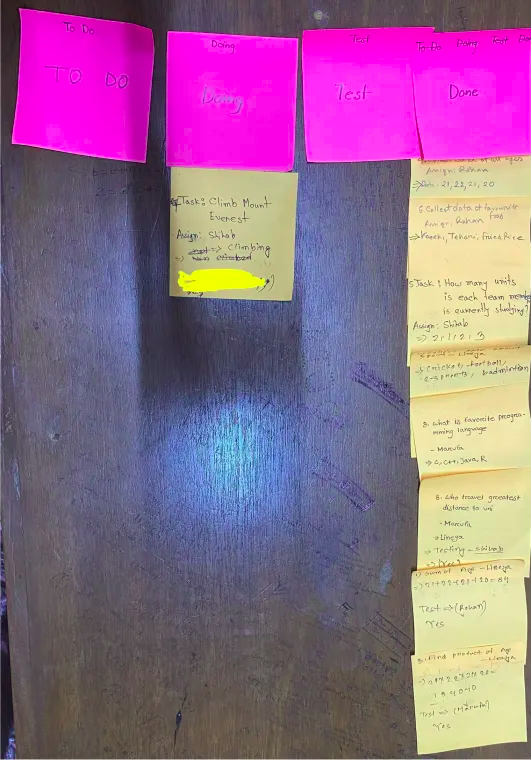
\includegraphics[width=0.5\linewidth]{figures/phase-5.png}
%    \caption{Phase 5}
%    \label{fig:placeholder}
%\end{figure}